%!TEX root = thesis.tex

\chapter{Proposed architecture}
\label{chapter:Proposed architecture}

Based on the aspects pointed out on Chapter~\ref{chapter:Payment terminal acceptance testing}, this part of the master's thesis will present a proposed architecture for automated acceptance testing environment for payment terminal software. Components of the environment can be divided into hardware and software components and this chapter is divided accordingly.

Research done in this master's thesis was carried out in co-operation with Eficode Oy and one of its customers providing payment terminal software in the Nordic countries. Motivation for this project came from the customer and Eficode Oy took responsibility of implementing the system according to the best practices of the industry. This proposal was initial plan for the project and it will be presented in this chapter.

\section{Overview}

When planning an automated acceptance test (AAC) environment for payment terminal software, environment has to be highly adaptive for different types of hardware and software features of different payment terminal models. This proposal was done for one payment terminal software provider and they had several different models of payment terminals and altogether 51 different software configurations for those devices.

Security is a top priority of payment terminal electronics and software and it is not possible to access internals of the payment terminal hardware. This means that AAC environment has to be able to manipulate the physical interface of the device. This also creates requirement for supporting different types of keyboard layouts and screen locations. In other words, environment has to be non dependent on single manufacturer or payment terminal model.

One of the requirements for the AAC environment was also use of open source technologies. For the reasons pointed out in Section~\ref{section:Open source}, customer wanted that the environment is as open as possible. This also creates reputation and visibility regarding the security matters.

Other requirements for the AAC environment was simplicity, low cost, low need for maintenance and ability to run the tests 24/7.

\section{Hardware}
\label{section:Proposed hardware}

Hardware for this proposal was intendedly kept simple and low-cost as possible. This proposal presents the use of just one Raspberry Pi 2 Mode B computer as a main computer for AAT environment (\emph{\cite{raspberry}}). Raspberry Pi 2 in relatively inexpensive compared to its computing power and it can also run full Linux operating system. It is small sized and does not require any cooling equipment. Therefore it suites well to this project as it can be situated easily to the environment and can be run over the clock without concerns about wearing cooling fans for example.

\FloatBarrier
\subsection{The Robot}
\label{subsection:The Robot proposal}

As internal electronics of the payment terminals are not accessible for security reasons, some sort of a robot is needed to be able to manipulate the physical UI of the payment terminals. Robot should therefore be able to accommodate different types of payment terminals and be able to press all types of buttons in question. Low cost and low need for maintenance are also requirements for this robot requested by the customer. Robot should also be able to manipulate multiple payment terminals at the same time in order to allow parallel execution of acceptance tests. This is intended to speed up the overall process as the same tests have to be run on different models of payment terminals. Other option would also be to make changing of the device under test easy and fast so that the manual work required can be minimized.

One of the options for automating the pressing of the buttons of the payment terminals would be to manufacture a frame on top the payment terminal which would have actuators for pressing each button. This would allow quick entering of key sequences and simultaneous pressing of multiple buttons. Hobby grade servo motors could be used as actuators in order to make this solution affordable. However, in order to support different kind of keyboard layouts and different sized payment terminals, the solution would require advanced mechanical engineering and thus the price of this solution could rise to become non cost-effective regarding the scope of this project and Master's Thesis. For these reasons this option for payment terminal manipulator is not proposed.

Other option for automatically pressing the buttons of the payment terminals would be utilizing the use of robotic arm. Robotic arm would be able to emulate a human user rather accurately and depending on the used robotic arm, simultaneous pressing of the buttons could also be possible. Drawback on the use robotic arm is the relatively high purchasing price of accurate and powerful robotic arms. This could be overcame by manufacturing the robotic arm with own resources and using some openly available plans (\emph{\cite{bcn3d}}) but this would require extensive use of time for building the arm from bottom up. For these reasons the use robotic arm is not proposed.

Third option for automating the key strokes of the payment terminal usage would be use of some kind of portal robot. For pressing of one key of the payment terminal at a time would need portal robot with at least 3 degrees of freedom. For the scope of this project and Master's Thesis this would be enough as it is only required to press one button of the payment terminal at a time. Portal robot would also be easily able to adapt to different kinds of keyboard layouts and payment terminal sizes as it can travel across any coordinates within its workspace. By choosing a portal robot with a right sized work space, if could be also possible to accommodate multiple payment terminals to the workspace at the same time. This would allow the execution of parallel acceptance tests within several different devices at the same time. For these reasons the use of portal robot for manipulating the buttons of the payment terminals is proposed.

The master's thesis proposes the use of ShapeOko 2 3-axis Computer Numerical Control (CNC) milling machine to be used as a manipulator (\emph{\cite{shapeoko}}). Though the machine is intended for milling purposes, it can be turned into a portal robot when milling tool is removed.

ShapeOko 2 is an open-source project and plans of the machine are openly available on their GitHub (\emph{\cite{shapeoko_git}}). This allows easy modifications to the hardware parts of the robot if needed.

ShapeOko 2 is controlled by an Arduino board running a program called GRBL (\emph{\cite{grbl}}). GRBL is an open source, high performance G-code interpreter and it is used for controlling CNC milling machines in general (\emph{\cite{shapeoko}}). G-code command are sent from Raspberry Pi 2 to the Arduino on the robot using serial communication.

Robot should be equipped with a pushing tool that can be manipulate the buttons. Pushing tool can be easily manufactured using for example 3D printing techniques.

\FloatBarrier
\subsection{Computer Vision Hardware}
\label{subsection:computer vision hardware}

In order to automate human interaction with the payment terminals, AAT environment has to be able to observe the changing content on the screen of the payment terminal. As stated earlier, internal electronics are not accessible due to the security measures and this disallows for example the possibly to hack the LCD communication line of the payment terminal in order to retrieve the image on the screen programmatically.

Therefore AAT environment also requires computer vision as changes on the screen have to observed visually. Manufacturer of Raspberry Pi offers low-price solution for this as a form of Raspberry Pi Camera Module (\emph{\cite{raspberry_camera}}). This module is proposed for use in computer vision tasks of the AAT environment.

As the size and the location of the display differs between different models of payment terminals, optical hardware has to be able to adapt to different kinds of imaging circumstances. As it is proposed that working area of the robot could be equipped with several payment terminals at the same time, also the displays of the payment terminals have to be able to be read regardless of the number of the devices under test.

One solution for this could be equipping the AAT environment with multiple stationary cameras, more precisely one camera per each device under test. If the cameras would be stationary this would create boundaries for the location and the size of payment terminal displays depending on the location of the optical hardware. Portal robot proposed also has rigid structure moving on top of the devices under test and this could cause blocking of the visual contact between camera and the display of the payment terminal.

Other solution would be having a moving camera that could be driven to a needed location in order to perform machine vision tasks. Location of the display could be configures regarding to the payment terminal model and this solution would adapt easily for different kinds of display layouts. Moving of the camera equipment can be achieved easily by attaching the camera directly to the portal robot. This will however exclude the ability to simultaneously pressing the buttons and reading the screen as robot has to be driven to certain position for capturing the image from the display. Regardless of this limitation, this solution is proposed. More precisely, it is proposed to situate the camera to the Z-axis assembly of the robot to the other side in respect to the pushing tool. This would minimize the required transitions when changing from pressing the buttons to capturing the images as the displays are typically located on top the numeric keypads on the payment terminals.

\FloatBarrier
\subsection{Card Feeder}
\label{subsection:Card feeder}

In addition to the manipulation of the payment terminal buttons, also the card feeding functionality has to be automated. One option to accomplish this functionality would be using the ShapeOko 2 robot for inserting and removing the card from the payment terminal. This would require some kind of a attachment to the payment card in order to make the manipulation of the card possible with the same tool that is used to push the buttons of the devices under test. In this case the AAT environment software would also require some kind of reset functionality in case the software would crash and the position of the card would be lost. Manipulation of the payment cards with the ShapeOko 2 robot would also make overall testing process slower as it would not be possible to press the buttons while inserting or removing the payment card to or from the payment terminal.

Other option would be manufacturing some kind of generally adaptable card feeders that could be used with different kinds of payment terminals. This solution would allow simultaneously inserting and removing of the payment card while manipulating the buttons with the robot. Advantage of this solution would also be that card feeders could know their state even if the software would crash and the reset functionality would be more simple to implement.

As insertion and removal of the credit card might be hard to accomplish in a simple way using just the robot described in previous section. This work proposes the use of generally designed card feeders to accomplish this task. Proposed card feeders consist of 3D printed base plate that attaches to the payment terminal, servo motor and 3D printed tray that attaches to the servo and to the credit card.

Card feeders are designed in a way that they can be used with any types payment terminals that have the card slot at the bottom edge of the device. Standard hobby servos are used as servo motors in order to keep the cost of the setup low.

Arduino board will be used to drive the servos as it can easily provide the needed pulse width modulated (PWM) signal for the servos. Arduino is suggested in order to ensure quality and accuracy of the PWM signal compared to what can be produced easily with non real time operating system running on the Raspberry Pi. Raspberry Pi on the machine will communicate with Arduino through serial communication.

\section{Software}
\label{section:software}

As stated in the Chapter \ref{subsection:Test syntax}, automated acceptance tests should be simple and understandable enough to actually make the automated testing efficient and beneficial. Open source solutions should be favored as this was requested by the customer and to achieve benefits described in the Chapter \ref{section:Open source} For these reasons software decisions of the AAT environment should be carefully considered in order to achieve good maintainability, compatibility and overall simplicity.

For software part of this AAC environment, Raspbian Wheezy is proposed for operating system. Raspbian is the official supported operating system for Raspberry Pi by Raspberry Pi Foundation (\emph{\cite{raspbian}}). Raspbian is based on widely used Debian Unix-like operating system. This allows the use of components developed for Debian to be used with this AAC environment.

\FloatBarrier
\subsection{Test Framework}
\label{subsection:test framework}

Based on the guidelines and comparison presented in Section \ref{section:test suite syntax}, the choice for test framework was consider in order to achieve the best usability, versatility and functionality. In order to maximize these measures, Robot Framework is proposed for the test framework. RF is an open-source, generic, keyword-driven test automation framework that has human readable test case syntax (\emph{\cite{Rfuserguide}}), (\emph{\cite{robotframework}}).

Robot Framework also has highly modular software architecture (\emph{\cite{Rfuserguide}}) and this allows the framework to be used with any kinds of testing libraries to connect to the system under test. This feature can be seen as a great advantage when implementing test libraries for machine control and computer vision (Chapter~\ref{subsection:test libraries}). Illustration of this modular architecture can be seen in Figure~\ref{fig:modular_architecture} bellow.

\begin{figure}[ht]
  \begin{center}
    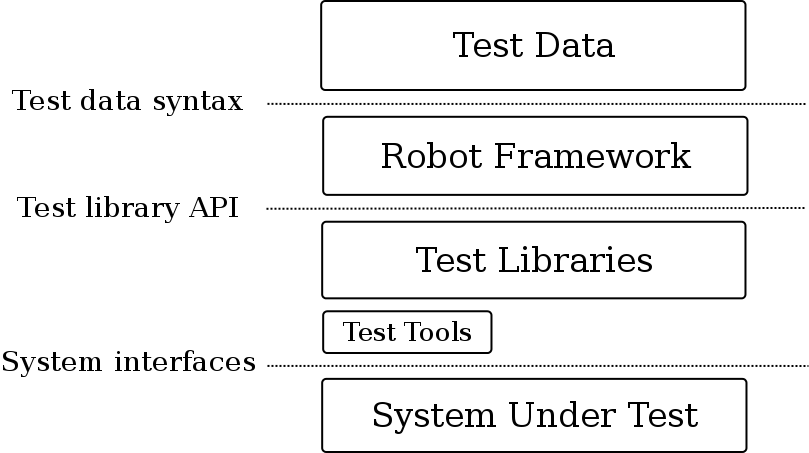
\includegraphics[width=8cm]{images/architecture-big.png}
    \caption{High level modular architecture. Source: \url{http://robotframework.org/img/architecture-big.png}}
    \label{fig:modular_architecture}
  \end{center}
\end{figure}

When RF tests are being run, it generates clear report and log files of the test case execution results (\emph{\cite{Rfuserguide}}). These files offer high level view of all test cases and step-by-step descriptions of individual test cases in order to make the debugging more easy.

Example of intended test case can be seen in Figure~\ref{fig:invalid_pin_test}. This test case describes automated RF acceptance test for entering invalid PIN code when trying to execute card purchase.

\begin{figure}[ht]
  \begin{center}
    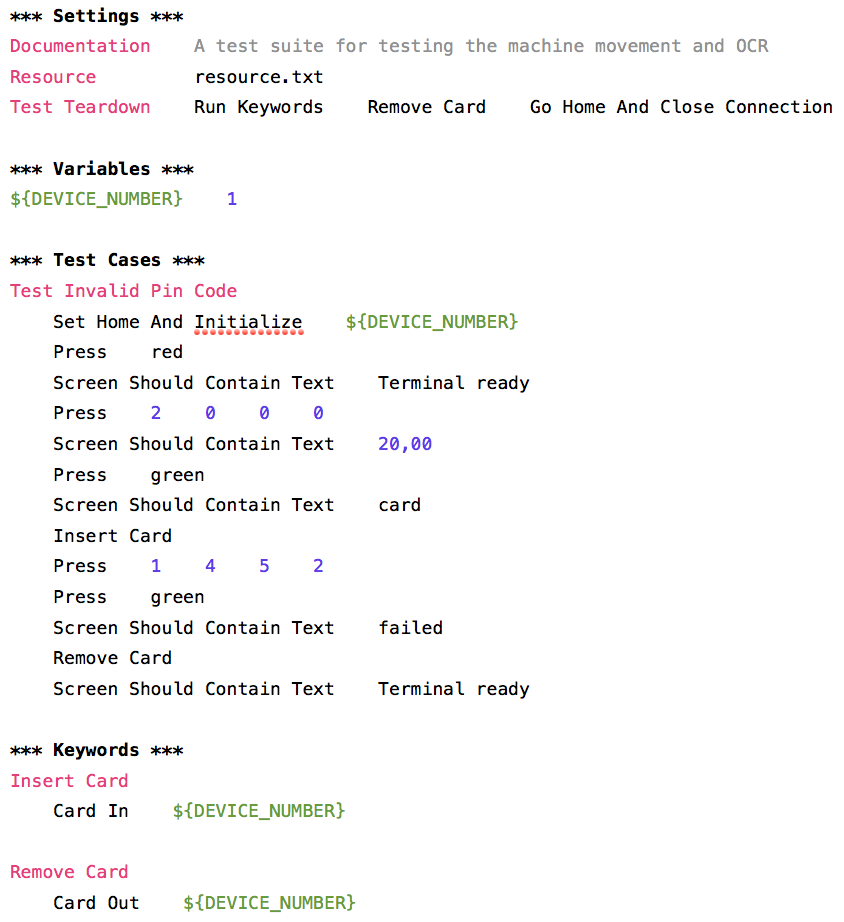
\includegraphics[width=10cm]{images/example_test.png}
    \caption{Example test case for invalid PIN code test}
    \label{fig:invalid_pin_test}
  \end{center}
\end{figure}

\FloatBarrier
\subsection{Test Libraries}
\label{subsection:test libraries}

As can be seen on Figure~\ref{fig:modular_architecture}, architecture requires external libraries to connect to the system under test. In the case of this AAT environment those libraries would be a library for machine control, a library for computer vision and a library for card feeder manipulation. All these libraries can be written using Python programming language that is supported out of the box by Robot Framework (\emph{\cite{robotframework}}).

For machine control library, the environment has to be able to send G-code command through USB serial communication to Arduino on the robot. For this pySerial Python library is proposed as it includes implementation of the needed serial communication functionalities (\emph{\cite{pyserial}}).

For the computer vision task of the environment, textual messages on the display are usually those that need to be verified. For this, character recognition is needed. Open source optical character recognition (OCR) engine called Tesseract OCR is proposed (\emph{\cite{tesseract}}). It was initially developed by HP but since 2006 it has been developed by Google. In order to use Tesseract OCR with Python, pytesseract wrapper is needed (\emph{\cite{pytesseract}}).

Library for controlling the card feeders is the most simplest one of these three libraries. For this, pySerial Python library is also proposed to send the serial communication command to the Arduino controlling the card feeders. Library will handle sending of control commands to the Arduino controlling the card feeder servo motors.